\section{Evaluation} \label{sec:evaluation}

\begin{figure*}[t]
\centering
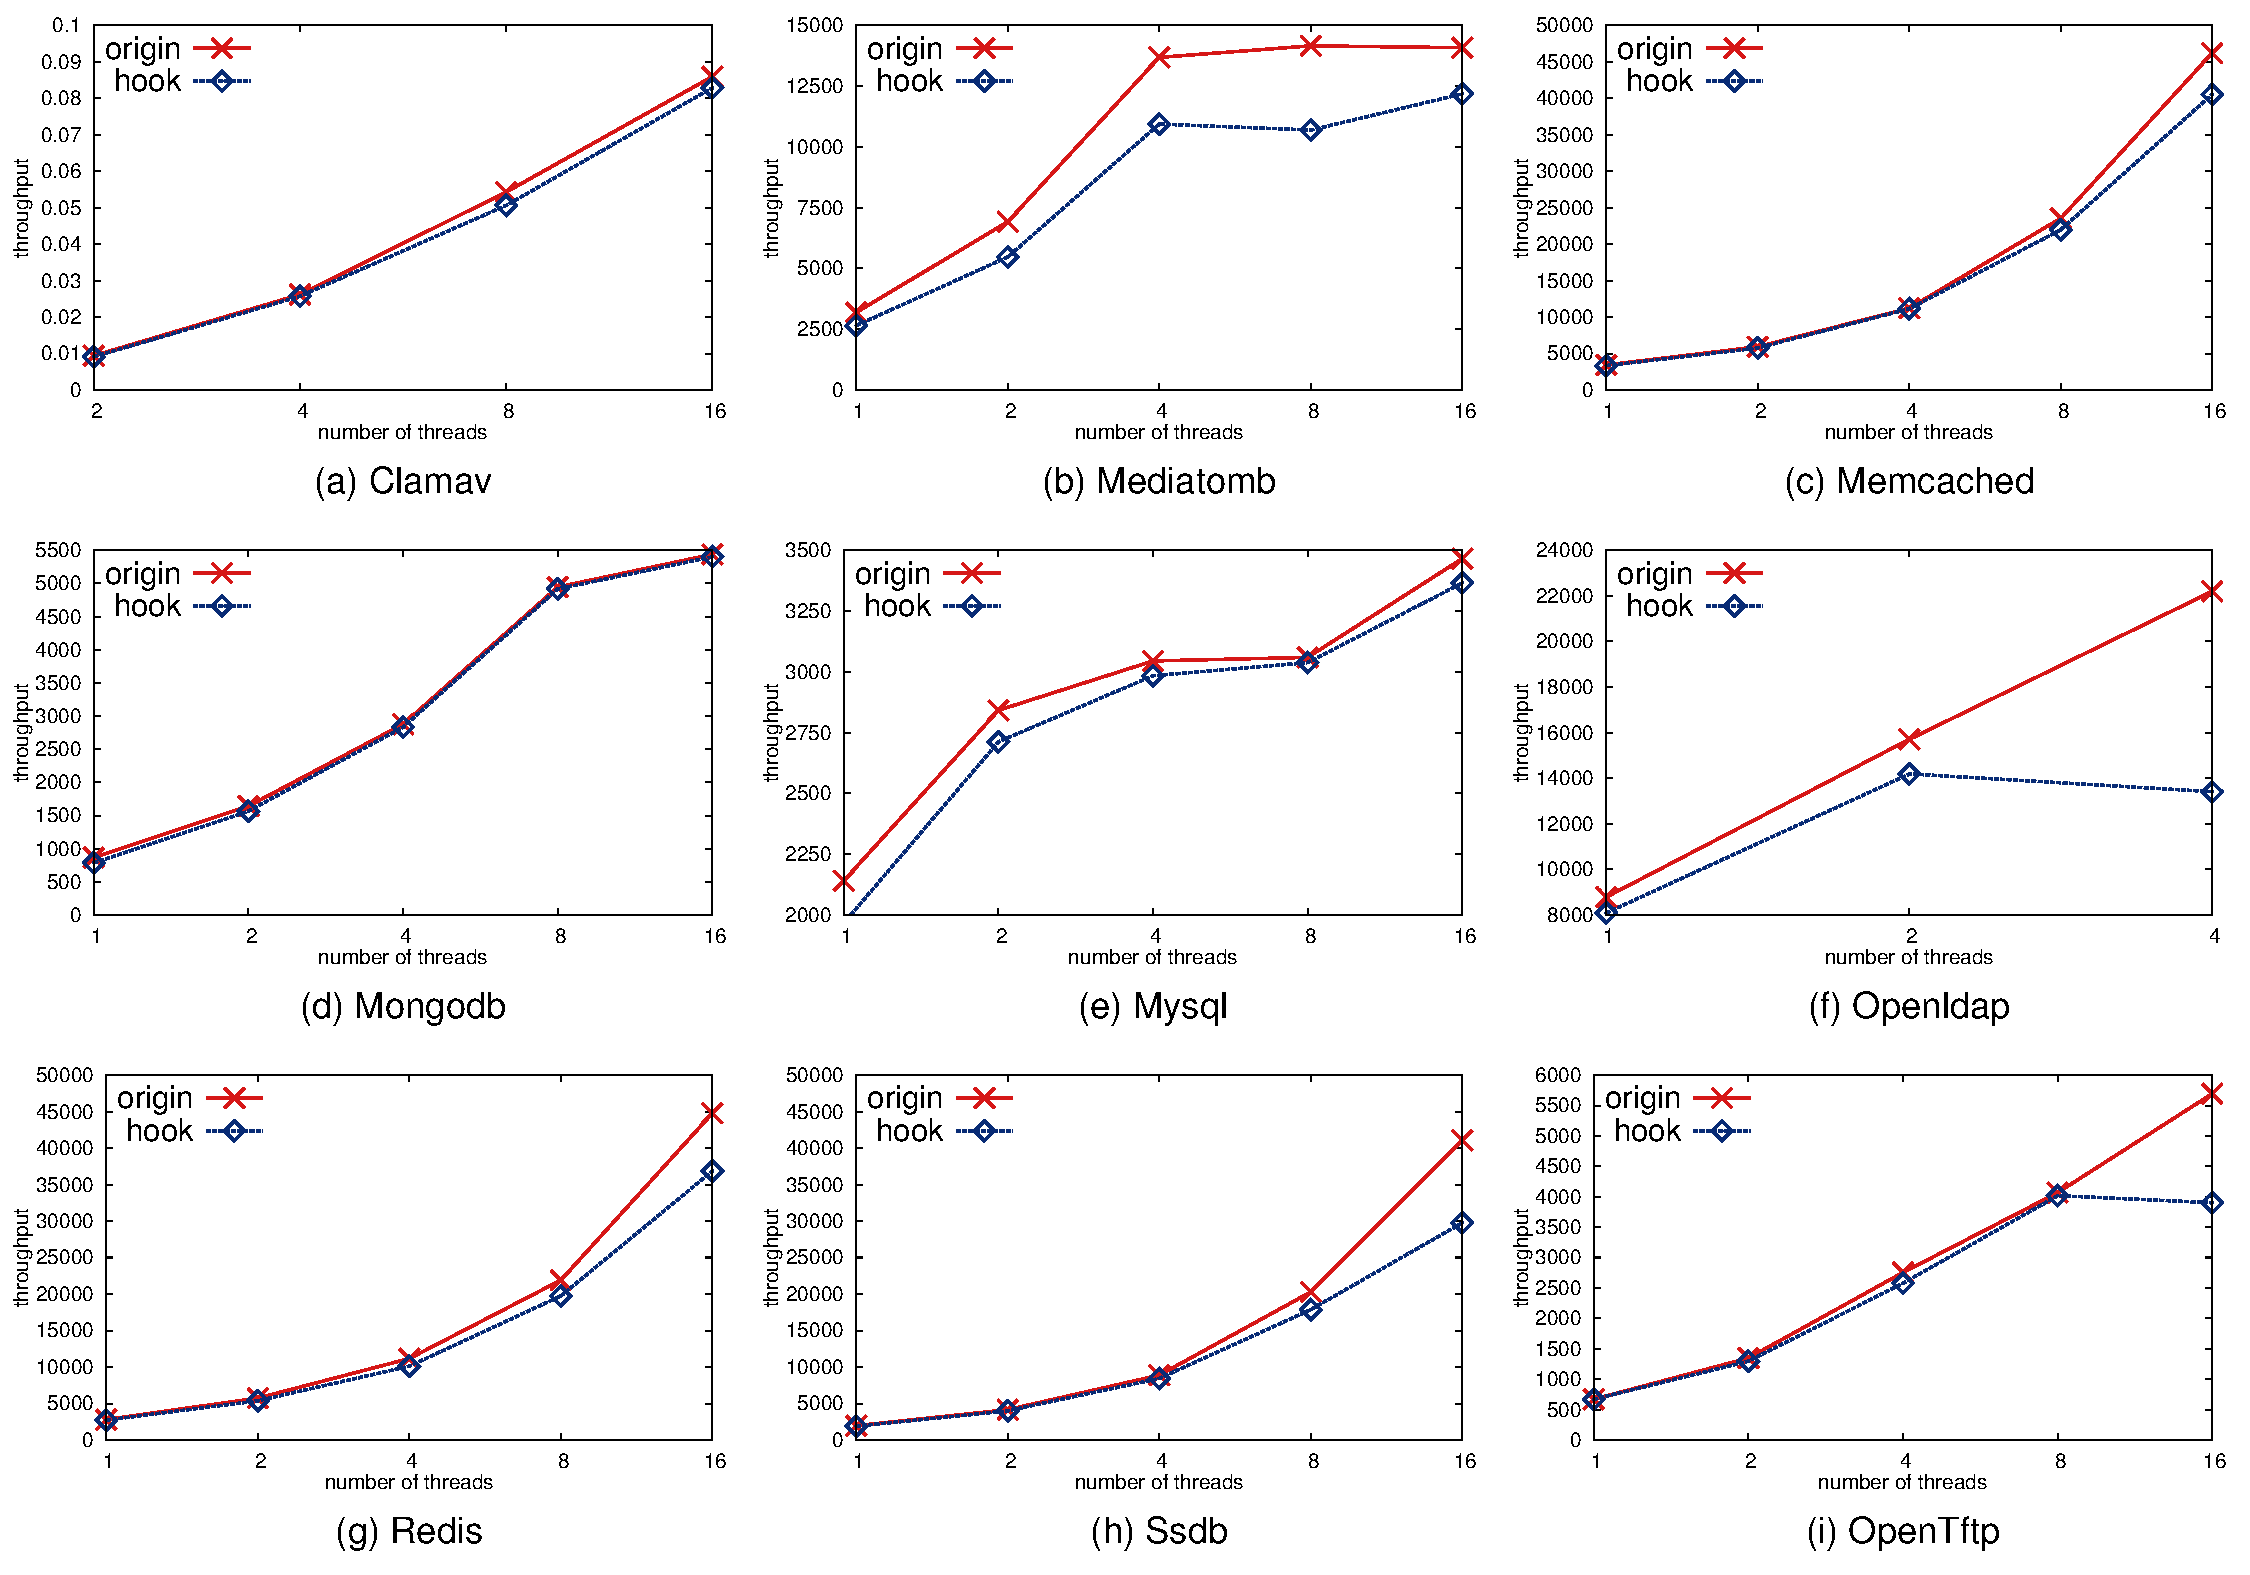
\includegraphics[width=0.9\textwidth]{figures/throughput}
\vspace{-.20in}
\caption{\small {\em \xxx throughput compared to the unreplicated 
execution.}}
\label{fig:tput}
\end{figure*}

\begin{figure*}[t]
\centering
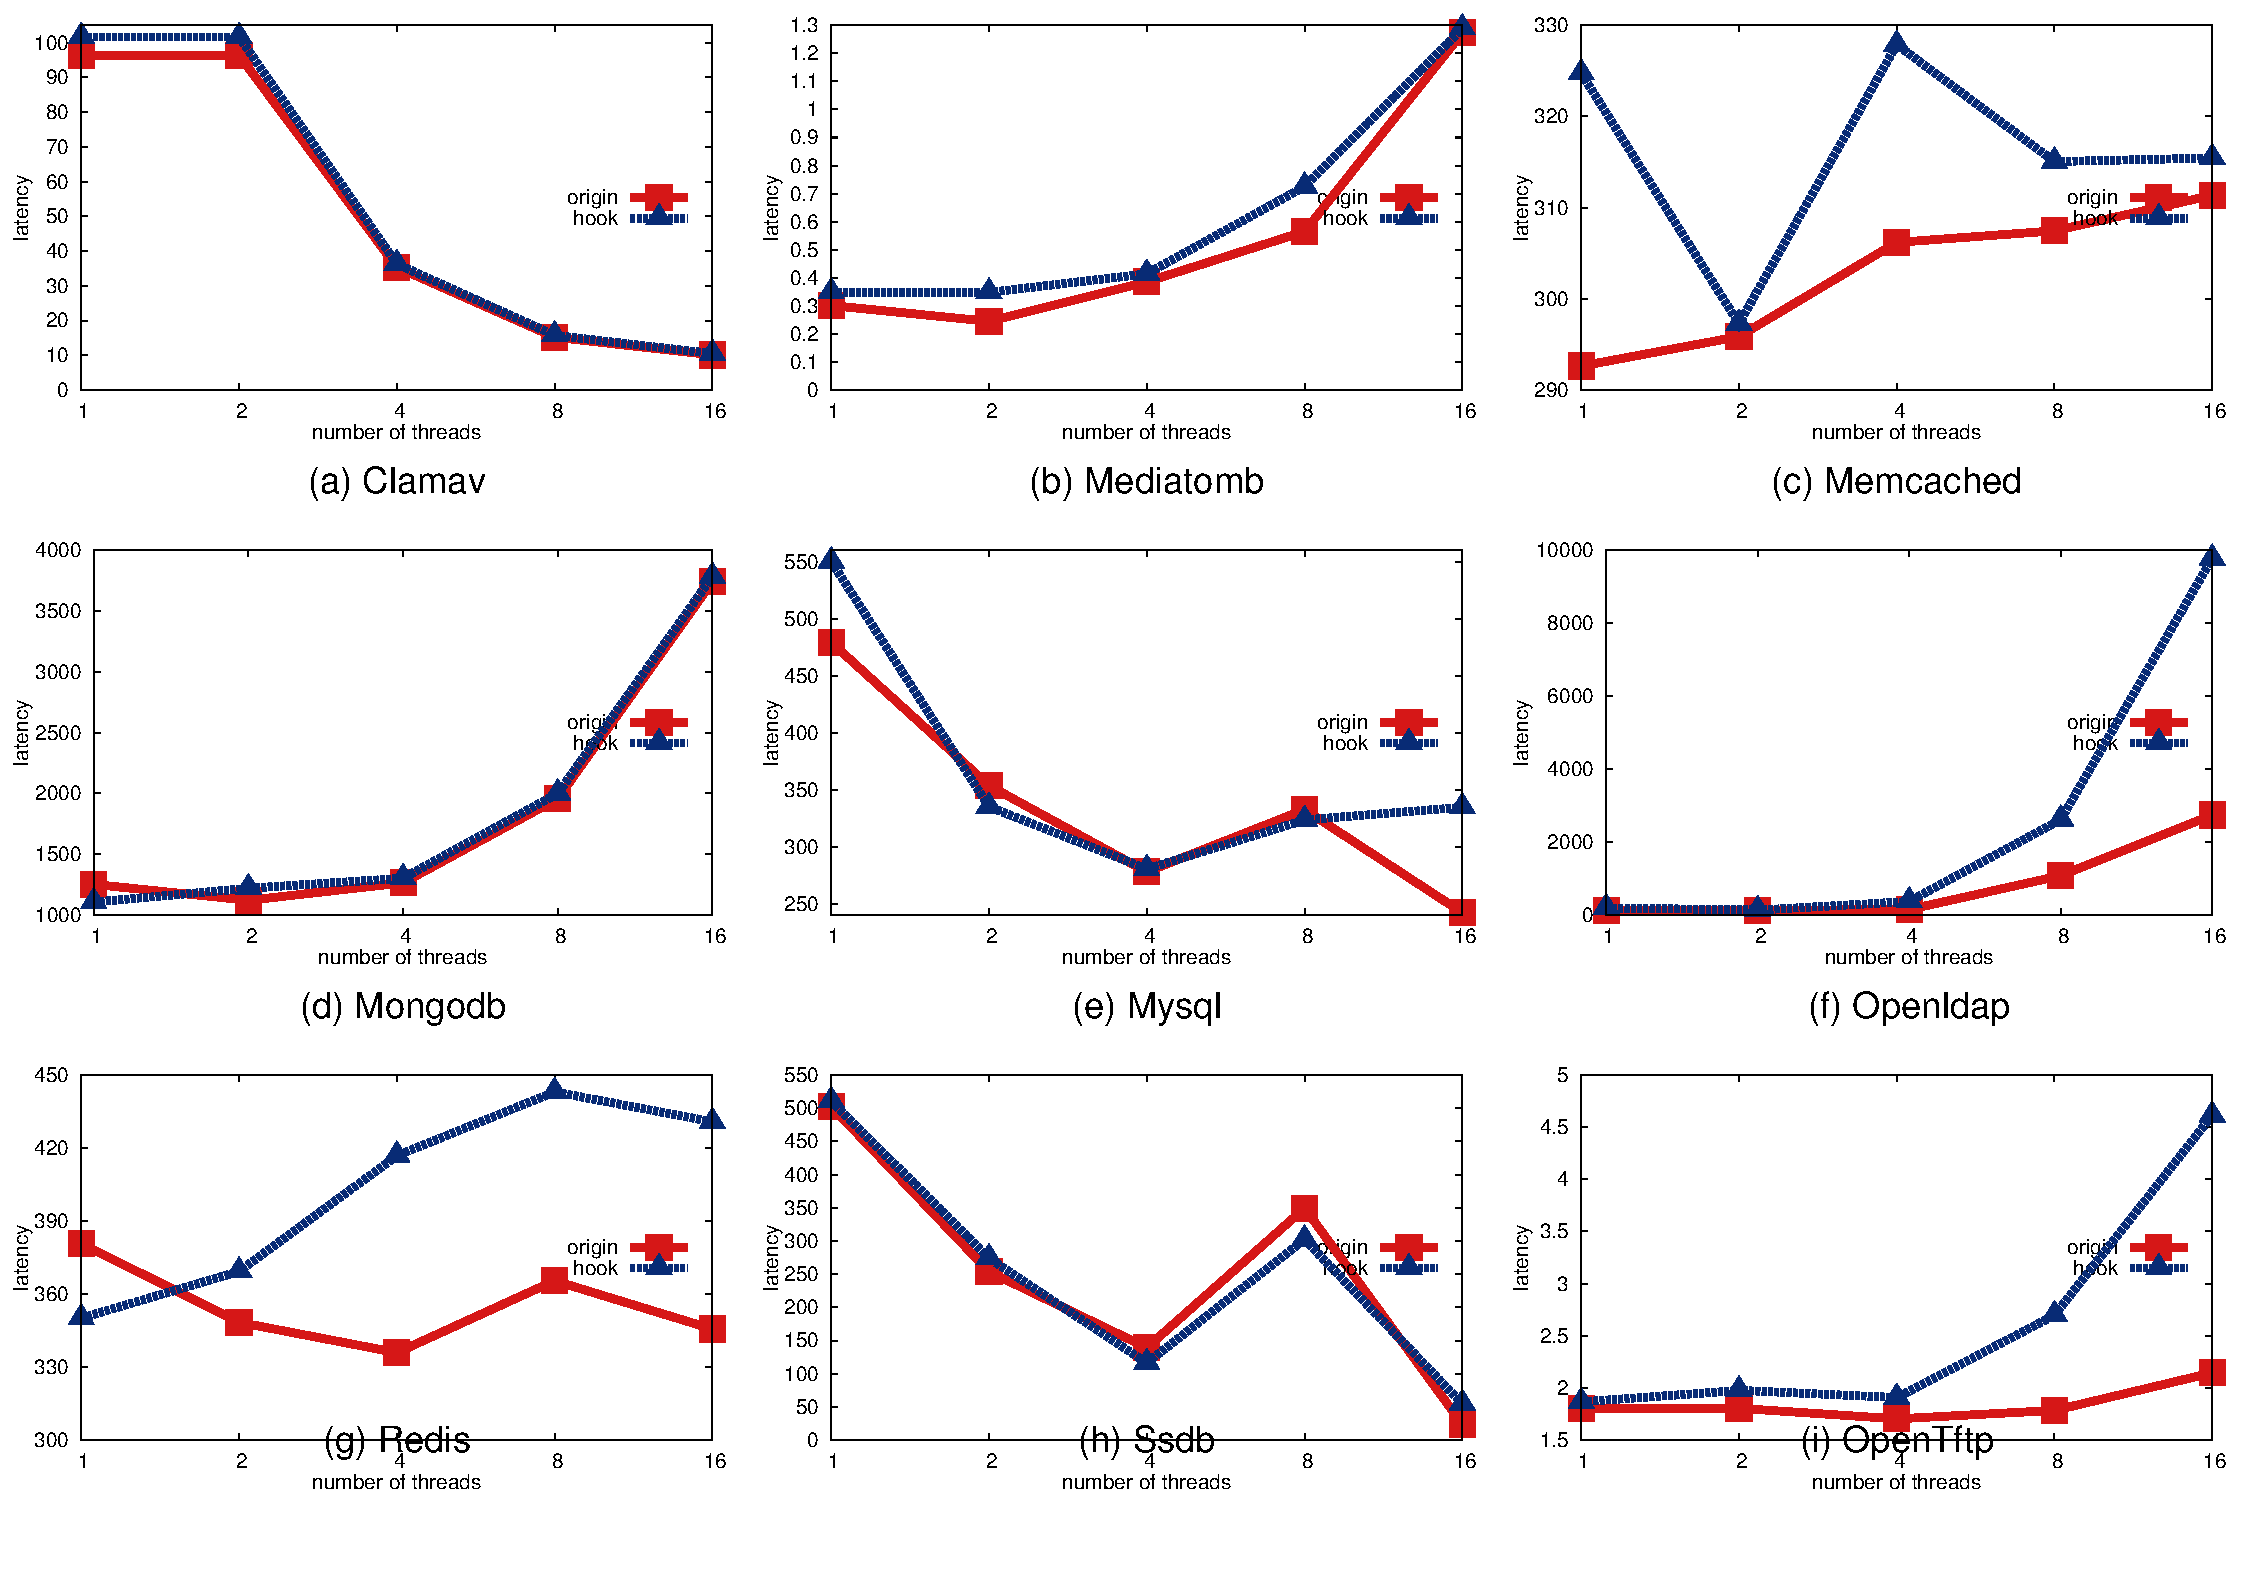
\includegraphics[width=0.9\textwidth]{figures/latency}
\vspace{-.20in}
\caption{\small {\em \xxx response time (latency) compared to the unreplicated 
execution.}}
\label{fig:latency}
\end{figure*}

Our evaluation used three Dell R430 servers as SMR replicas. Each server having 
Linux 3.16.0, 2.6 GHz Intel Xeon CPU with 24 hyper-threading cores, 32GB 
memory, and 1T SSD. Each machine has a Mellanox ConnectX-3 Pro Dual Port 40 Gbps 
NIC. These NICs are connected using the Infiniband RDMA architecture through a 
Dell S6000 high-performance switch with 32 40Gpbs ports. The \v{ping} latency 
between every two replicas are 84 \us. This latency is achieved through IPoIB 
(IP over Infiniband), the optimal latency for a client to communicate with a 
server through traditional TCP/IP.

To mitigate network latency of public network, all client benchmarks were ran 
in a Dell R320 server, with Linux 3.16.0, 2.2GHz Intel Xeon with 12 
hyper-threading cores, 32GB memory, and 160G SSD. This server connects with the 
replica machines with 1Gbps bandwidth LAN, with a mean 301 \us \v{ping} 
latency. A larger network latency (\eg, sending client requests from WAN) will 
further mask \xxx's overhead.

We evaluated \xxx on \nprog widely used or studied server programs, including 
\nkvprog key-value stores \redis, \memcached, \ssdb, \mongodb; \mysql, a SQL 
server; \clamav, a anti-virus server that scans files and delete malicious ones; 
\mediatomb, a multimedia storage server that stores and transcodes video and 
audeo files; \openldap, an LDAP server; \calvin, a widely studied transactional 
database system that leverages \zookeeper as its SMR service. All these programs 
are multithreaded except \redis (but it can still serve requests concurrently 
using Libevent). These servers all update or store important data and files, 
thus the high fault-tolerance of SMR is especially attractive to these programs.

\begin{table}[b]
\footnotesize
\centering
\vspace{-.05in}
\begin{tabular}{lrr}
{\bf Program} & {\bf Benchmark} & {\bf Benchmark workload description}\\
\hline\\[-2.3ex]
\clamav & Self  & Scan files in \v{/usr/lib} directory \\
\mediatomb & ApacheBench  & Transcode video files in parallel\\
\memcached & mcperf  & 50\% set and 50\% put operations\\
\mongodb & YCSB  & Workload C\\
\mysql & Sysbench  & Concurrent SQL transactions\\
\openldap & Self  & TBD\\
\redis & Self  & 50\% set and 50\% put operations\\
\ssdb & Self  & 50\% set and 50\% put operations\\
\calvin & Self  & Concurrent SQL transactions\\
\end{tabular}
\vspace{-.05in}
\caption{{\em Benchmarks and workloads.} ``Self" in the Benchmark column means 
we used a server program's own performance benchnmark.} 
\label{tab:benchmarks}
\end{table}


% Benchmarks table.
Table~\ref{tab:benchmarks} introduces the benchmarks and workloads we used. To 
evaluate \xxx's practicality, we used the server developers' own performance 
benchmarks or popular third-party. For benchmark workload settings, we used the 
benchmarks' default workloads whenever available. We spawned 
up to 16 concurrent connections which made these servers approach peak 
throughput, and then we measured both response time (latency) and throughput. We 
also measured \xxx's bare consensus latency. Each performance data point in the 
evaluation is taken from the mean value of 10 repeated executions.

% evaluation metric. client benchmarks all run in LAN, average latency
The rest of this section focuses on these questions:

\begin{tightenum}

\item[\S\ref{sec:ease-of-use}:] How easy is it to run general server programs 
in \xxx?

\item[\S\ref{sec:overhead}:] What is \xxx's performance compared to the 
unreplicated executions? What is \xxx's network latency on input coordination 
and output checking?

\item[\S\ref{sec:scalability}:] How scalable is \xxx on different sizes of 
replica group?

\item[\S\ref{sec:compare}:] What is \xxx's performance compared to existing 
SMR systems?

\item[\S\ref{sec:robust}:] How fast can \xxx recover replicas from output 
divergence?

% \item[\S\ref{sec:race}:] If some \xxx users care about data races much, how 
% does \xxx tolerate the slowdown of data race detector by deploying it on a 
% replica?

% \item[\S\ref{sec:lesson}:] What practical lessons have we learnt during the 
% case study on these server programs with \xxx?

\end{tightenum}

\subsection{Ease of Use} \label{sec:ease-of-use}

\xxx is able to run all \nprog evaluated programs without modifying them 
except for \calvin. \calvin integrates its client program and server program 
within the same process and uses memory to send transactions from the 
client to server. We wrote a \nlinescalvin patch to separate the client 
and server and make them communicate with POSIX sockets.

\subsection{Performance Overhead} \label{sec:overhead}

\begin{table}[b]
\footnotesize
\centering
\vspace{-.05in}
\begin{tabular}{lrrrrr}
{\bf Program} & {\bf \# calls} & {\bf input} & {\bf SSD} 
& {\bf quorum} & {\bf diff}\\
\hline\\[-2.3ex]
\clamav & 30  & 42.0 & 5.1 \us & 6.1 \us & F\\
\mediatomb & 3,000  & 140.0 & 4.7 \us & 5.8 \us & F?\\
\memcached & 10,016  & 38.0 & 4.9 \us & 6.9 \us & F?\\
\mongodb & 25,665  & 492.4 & 19.1 \us & 20.4 \us & F?\\
\mysql & 13,111  & 26.0 & 5.0 \us & 15.7 \us & W?\\
\openldap & 8,040  & 27.3 & 5.7 \us & 7.1 \us & T\\
\redis & 10,016  & 107.0 & 3.6 \us & 6.3 \us & T\\
\ssdb & 9,916  & 47.0 & 3.7 \us & 10.9 \us & F*\\
\calvin & TBD  & TBD & TBD  & TBD & TBD\\
\end{tabular}
\vspace{-.05in}
\caption{{\em \xxx micro events.} The ``\# Calls" column means the number of 
socket calls that went through \xxx input concensus; ``input" means average 
bytes of a server's inputs received in these calls; ``SSD" means the average 
latency on storing these calls to stable storage; ``quorum" means the
average latency on waiting quorum for these calls; and ``diff" means whether 
the output checker found output divergence.} 
\label{tab:consensus-latency}
\end{table}

We ran all the evaluated server programs in \xxx with a replica group size of 
three, and varied the number of threads in each server program by up to 16 
threads or until they reached peak performance. Figure~\ref{fig:tput} shows 
\xxx's throughput. The average througput degrades only \tputoverhead for all 
these server programs because of two reasons. First, \xxx's input coordination 
protocol only contains two one-sided RDMA writes and two SSD writes between 
each leader-backup pair. XXX. Second, \xxx's output checking protocol only 
involes for every \thashcomp output hash generations, which is pretty sparse 
compared to input coordination.
% Overhead compared with unreplicated executions.


Figure~\ref{fig:latency} shows \xxx's latency.
% Bare consensus latency, micro events.

\subsection{Scalability on Replica Group Size} \label{sec:scalability}

TBD.
% 3, 5.

\subsection{Comparison with Traditional SMR systems} \label{sec:compare}

TBD.
% Run Calvin on Zookeeper, Crane, and Falcon. Because we can only make Calvin's 
% database with Zookeeper. XX speedup.

\subsection{Recovering from Output Divergence} \label{sec:robust}

TBD.
% Change 

% 
% \subsection{Sensitivity of Parameters} \label{sec:sensitivity}

% Change output comparison periods. 1, 100, 1000, 10000. 1000 is the smallest 
% number that starts to have negligible overhead. Run only with the server with 
% largest recv() data size.

% Twait

% Tcomphash
 
% \subsection{Read-only Optimization} \label{sec:read-opt}

% % 